%!TEX root = main.tex
%%% Exponentials & Logarithms
\part{}

\section{Inverse Functions}

Consider the composition of the following two functions.
\[
f(x)=x+300\qquad g(x)=x-300
\]
\begin{solution}[2.25in]

\end{solution}

\vspace{0.5em}

\begin{definition}\label{def: inverses}
If for two functions $f(x)$ and $g(x)$, $(g\circ f)(x)=\blank{x}{x}$ \&
$(f\circ g)(x)=\blank{x}{x}$ for all $x$ in their domains,
then we call $g(x)$ the \emph{inverse of }$f(x)$ denoted $f^{-1}(x)$.
\end{definition}

\vspace{0.5em}

\begin{exercise}
Verify that $f(x)=4x-7$ and $\dl g(x)=\frac{x+7}{4}$ are inverses.
\end{exercise}
\begin{solution}[4in]

\end{solution}

\vspace{0.5em}

\begin{exercise}
Verify that $f(x)=-2x-1$ and $\dl g(x)=\frac{-x}{2}-\frac{1}{2}$ are inverses.
\end{exercise}
\begin{solution}[4in]

\end{solution}

\subsection{Finding Inverses}

\begin{example}
Let's deduce the inverse for $f(x)=3x+2$
\end{example}

\ifprintanswers\else\newpage\fi

\subsection{Algebraically finding the inverse}

Here are the steps for calculating the inverse

\begin{enumerate}[1)]
    \item Replace $f(x)$ by $y$
    \item Interchange (``switch'') the $x$'s and $y$'s
    \item Solve for $y$
    \item Replace $y$ by $f^{-1}(x)$
\begin{enumerate}
    \item[4.5] Verify by composing the two functions 
\end{enumerate}
\end{enumerate}

\vspace{0.5em}

\begin{exercise}
Find the inverse of $f(x)=2x+7$
\end{exercise}
\begin{solution}[2in]

\end{solution}

\begin{exercise}
Find the inverse of $\dl f(x)=\frac{9x-7}{4x+3}$
\end{exercise}
\begin{solution}[4in]

\end{solution}

\begin{exercise}
Find the inverse of $\dl f(x)=\frac{2x+3}{4x-7}$
\end{exercise}
\begin{solution}[4in]

\end{solution}

\begin{exercise}
Find the inverse of
\[
f(x)=-9\sqrt{x-8}+5
\]
for $x\geq8$
\end{exercise}
\begin{solution}[3in]

\end{solution}

\begin{note}
Notice that since we switch the $x$'s and $y$'s when finding
the inverse, it makes sense that
\[
\blank{f(a)=b}{f(a)=b}\leftrightarrow\blank{f^{-1}(b)=a}{f^{-1}(b)=a}
\]
\end{note}

\begin{exercise}
Based on the following table of values for $f(x)$. Find the requested values of $f^{-1}(x)$.
\begin{center}
\begin{tabular}{c|c|c|c|c|c|c}
$x$ & $1$ & $3$ & $7$ & $9$ & $11$ & $12$ \\\hline
$f(x)$ & $-5$ & $1$ & $2$ & $4$ & $8$ & $10$ 
\end{tabular}
\end{center}
\begin{itemize}
    \item $f^{-1}(1)=$
    \item $f^{-1}(-5)=$
    \item $f^{-1}(8)=$
\end{itemize}
\end{exercise}

\subsection{Finding inverses graphically}

\begin{prop}[Horizontal Line Test]\label{prop: HLT}
A function $f(x)$ has an inverse, $f^{-1}(x)$, if no horizontal
line crosses its graph more than once.
\end{prop}

\begin{center}

\begin{tikzpicture}[scale=0.5]
\draw[step=1cm,gray,very thin] (-5,-5) grid (5,5);
\draw (-5,0) -- (5,0);
\draw (0,-5) -- (0,5);
\end{tikzpicture}
\hspace{1in}

\begin{tikzpicture}[scale=0.5]
\draw[step=1cm,gray,very thin] (-5,-5) grid (5,5);
\draw (-5,0) -- (5,0);
\draw (0,-5) -- (0,5);
\end{tikzpicture}
\end{center}

\begin{definition}
We call functions that pass the Horizontal Line Test \emph{one-to-one}
\end{definition}

\subsection{Finding the graph}

\begin{exercise}
Find the graph of $f^{-1}(x)$ if $f(x)$ is given below
\begin{center}
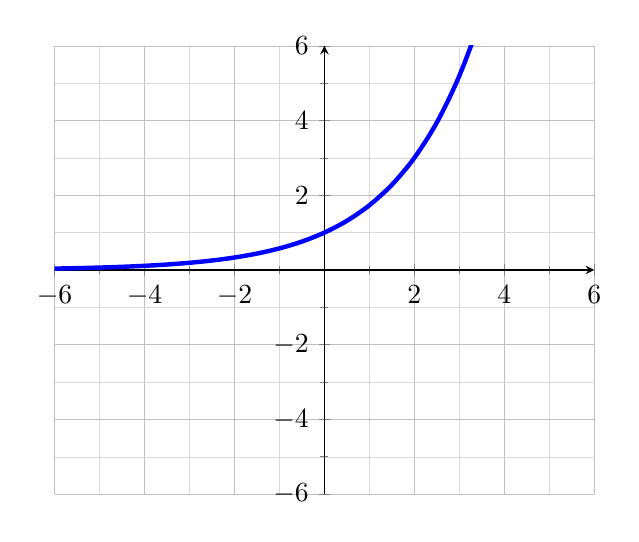
\begin{tikzpicture}
\begin{axis}%
    [grid=both,
     minor tick num=1,
     ymin=-6, ymax=6,
     xmin=-6, xmax=6,
     grid style={line width=.1pt, draw=gray!30},
     major grid style={line width=.2pt,draw=gray!50},
     axis lines=middle,
     enlargelimits=false,
    ]
    \addplot[domain=-6:6, blue, ultra thick,smooth] {3^(0.5*x)};
\end{axis}
\end{tikzpicture}
\end{center}
\end{exercise}

\begin{exercise}
Find the graph of $f^{-1}(x)$ if $f(x)$ is given below
\begin{center}
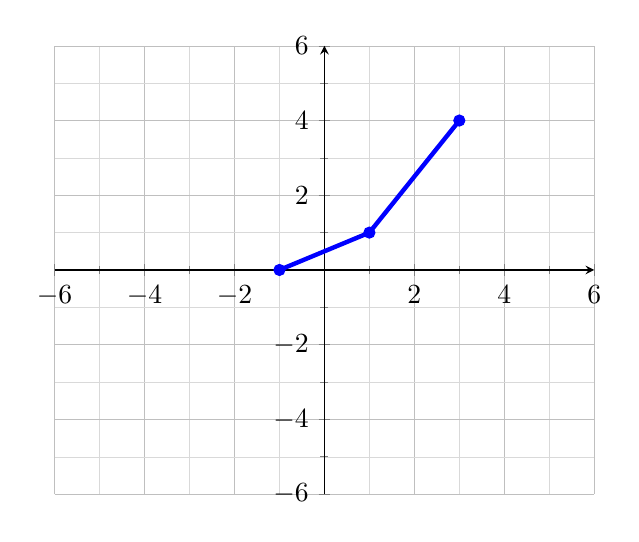
\begin{tikzpicture}
\begin{axis}%
    [grid=both,
     minor tick num=1,
     ymin=-6, ymax=6,
     xmin=-6, xmax=6,
     grid style={line width=.1pt, draw=gray!30},
     major grid style={line width=.2pt,draw=gray!50},
     axis lines=middle,
     enlargelimits=false,
    ]
    \addplot[domain=-1:1, blue, ultra thick, smooth] {0.5*x+0.5};
    \addplot[domain=1:3, blue, ultra thick, smooth]{3/2*x-0.5};
    \addplot[only marks, blue] coordinates {(-1,0) (1,1) (3,4)};
\end{axis}
\end{tikzpicture}
\end{center}
\end{exercise}

\subsection{Restricting the domain}
\begin{example}
Consider the function $f(x)=x^2$
\begin{center}
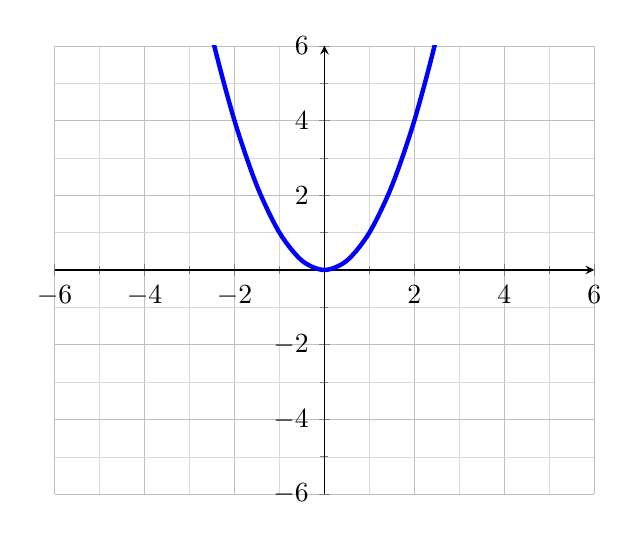
\begin{tikzpicture}
\begin{axis}%
    [grid=both,
     minor tick num=1,
     ymin=-6, ymax=6,
     xmin=-6, xmax=6,
     grid style={line width=.1pt, draw=gray!30},
     major grid style={line width=.2pt,draw=gray!50},
     axis lines=middle,
     enlargelimits=false,
    ]
    \addplot[domain=-6:6, blue, ultra thick, smooth] {x^2};
\end{axis}
\end{tikzpicture}
\end{center}
\end{example}
\vspace{2em}

\ifprintanswers\else\newpage\fi

\begin{exercise}
How could we restrict the domain of the following function
to make it one-to-one?
\begin{center}
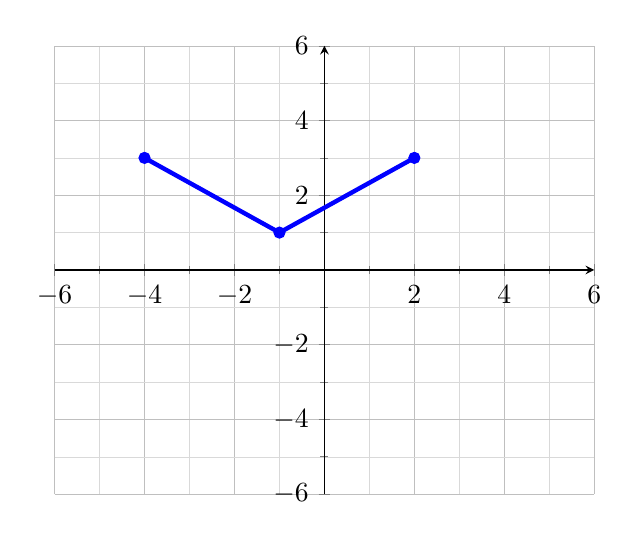
\begin{tikzpicture}
\begin{axis}%
    [grid=both,
     minor tick num=1,
     ymin=-6, ymax=6,
     xmin=-6, xmax=6,
     grid style={line width=.1pt, draw=gray!30},
     major grid style={line width=.2pt,draw=gray!50},
     axis lines=middle,
     enlargelimits=false,
    ]
    \addplot[domain=-4:-1, blue, ultra thick, smooth] {-2/3*(x+1)+1};
    \addplot[domain=-1:2, blue, ultra thick, smooth] {2/3*(x+1)+1};
    \addplot[only marks, blue] coordinates {(-4,3) (-1,1) (2,3)};
\end{axis}
\end{tikzpicture}
\end{center}
\end{exercise}
\begin{solution}[1in]

\end{solution}
\section{Exponential Functions}

\begin{definition}\label{def: exponential func}
A (basic) \emph{exponential function} can be written as follows
\[
f(x)=\blank{a(b)^x}{a(b)^x}
\]
where $\blank{b}{b}$ is called the base and $\blank{b>0~\&~b\neq1}{b>0~\&~b\neq1}$
\end{definition}
\vspace{1em}

\begin{example}
\text{}
\begin{itemize}
    \item $f(x)=\blank{\dl-7\left(\frac{1}{5}\right)^x}{\dl-7\left(\frac{1}{5}\right)^x}$
    \item $f(x)=\blank{(1.5)^x}{(1.5)^x}$
    \item $f(x)=\blank{(2)^{x-7}}{(2)^{x-7}}$
\end{itemize}
\end{example}

\vspace{0.5em}

\begin{nonex}
\text{}
\begin{itemize}
    \item $f(x)=\blank{7(-3)^x}{7(-3)^x}$
    \item $f(x)=\blank{x^8}{x^8}$
\end{itemize}
\end{nonex}

\vspace{0.5em}

\begin{exercise}
Let $\dl f(x)=\frac{1}{2}(4)^{x-1}$. Evaluate $f(3)$ without a calculator.
\end{exercise}
\begin{solution}[4in]

\end{solution}

\begin{exercise}
Let $\dl f(x)=3\left(\frac{1}{2}\right)^{x+1}$. Find $f(1)$.
\end{exercise}
\begin{solution}[4in]

\end{solution}

\begin{exercise}
Let $\dl f(x)=-8\left(2\right)^{3x}+3$. Evaluate $f(0)$.
\end{exercise}
\begin{solution}[2.5in]

\end{solution}

\subsection{Finding the equation}

\subsubsection*{Initial point/value is known}

\begin{exercise}
Construct an exponential function that contains $(0,-2)$ \& $(3,-128)$.
\end{exercise}
\begin{solution}[5in]

\end{solution}


\begin{exercise}
The graph of an exponential function has a $y$-intercept of $7$ and contains the point
$(4,112)$. Find the equation.
\end{exercise}
\begin{solution}[4in]

\end{solution}

\subsubsection*{Initial point/value is unknown}

\begin{exercise}
Find the exponential function that contains $(2,48)$ \& $(3,192)$.
\end{exercise}
\begin{solution}[3.5in]

\end{solution}

\begin{exercise}
Find the exponential function that contains $(1,300)$ \& $(2,100)$.
\end{exercise}
\begin{solution}[4in]

\end{solution}

\subsection{Word problems}

\begin{exercise}
The number of users online at a website has grown exponentially since its launch.
After 2 months, there are 200 users. After 4 months, there are 800 users. Find the
function that models the number of users $x$ months after launch.
\end{exercise}
\begin{solution}[3.5in]

\end{solution}

\begin{exercise}
The selling price of a car is \$13,500. Each year it loses 11\% of its value.
Find the exponential that models its value after $x$ years.
\end{exercise}
\begin{solution}[5in]

\end{solution}

\subsection{Compound Interest}

\begin{prop}[Compound Interest Formula]
If an initial investment of $P$ (typically referred to as \emph{principle})
at an interest rate of $r$ compounded $n$ times a year, then the amount after $t$
years would be
\[
A=\blank{P\left(1+\frac{r}{n}\right)^{nt}}{P\left(1+\frac{r}{n}\right)^{nt}}
\]
\end{prop}

\ifprintanswers\else\newpage\fi

\begin{exercise}
If \$5000 is borrowed at an interest rate of 12.3\% compound semi-annually, what
is the total amount of money needed to pay it back in 3 years? Round to nearest dollar.
\end{exercise}
\begin{solution}[3.5in]

\end{solution}

\begin{exercise}
A loan is paid off in 15 years with a total of \$192,000. If it had a 4\% interest rate
compounded monthly, what was the initial amount borrowed?
\end{exercise}
\begin{solution}[3.5in]

\end{solution}

\subsection{The Natural Number}

\begin{definition}\label{def: eulars constant}
\emph{Euler's Constant} (or the \emph{Natural Number}) is a special constant
denoted by the letter $e$. It can be found as follows
\[
\blank{(1+\frac{1}{n})^n\xrightarrow[n\rightarrow\infty]{e}}{(1+\frac{1}{n})^n\xrightarrow[n\rightarrow\infty]{e}}
\]
\end{definition}

\begin{exercise}
For $f(x)=-7e^x$, find $f(2)$ rounded to one decimal place.
\end{exercise}
\begin{solution}[3in]

\end{solution}

\subsection{Continuous growth or decay}

\begin{prop}
Something that is changing continuously either growing or decaying can be modeled 
as follows:
\[
A=\blank{Pe^{rt}}{Pe^{rt}}
\]
Where $P$ is the initial amount, $r$ is the rate of change ($r<0$ means it is decaying
and $r>0$ if it is growing), and $t$ is the amount of time passed. 
\end{prop}

\ifprintanswers\else\newpage\fi

\begin{exercise}
A motorcycle bought at \$10,000 depreciates continuously at 9\% per anum.
What is its value after 7 years?
\end{exercise}
\begin{solution}[3in]

\end{solution}

\subsection{Graphs of Exponentials}

The base $b$ of an exponential $b>1$ or $0<b<1$ which have two respective styles
of graphs:

\begin{center}

\begin{tikzpicture}[scale=0.6]
\draw[step=1cm,gray,very thin] (-5,-5) grid (5,5);
\draw (-5,0) -- (5,0);
\draw (0,-5) -- (0,5);
\end{tikzpicture}
\hspace{0.5in}

\begin{tikzpicture}[scale=0.6]
\draw[step=1cm,gray,very thin] (-5,-5) grid (5,5);
\draw (-5,0) -- (5,0);
\draw (0,-5) -- (0,5);
\end{tikzpicture}
\end{center}

\ifprintanswers\else\newpage\fi

\subsubsection*{Characteristics of basic exponentials}

If the we have a basic exponential $f(x)=b^x$, it has the following properties:
\begin{enumerate}[1)]
    \item $D_f:\blank{(-\infty,\infty)}{(-\infty,\infty)}$ \& $R_f:\blank{(0,\infty)}{(0,\infty)}$
    \item $y$-intercept: $\blank{(0,1)}{(0,1)}$ \& $x$-intercept: \blank{DNE}{DNE}
    \item If $b>1$, \blank{$f$ is increasing}{$f$ is increasing}. If $0<b<1$, \blank{$f$ is decreasing}{$f$ is decreasing}.
    \item $f(x)$ is \blank{one-to-one}{one-to-one}, so
    \blank{it has an inverse}{it has an inverse}.
    \item $f$ has a Horizontal Asymptote at $\blank{y=0}{y=0}$.
\end{enumerate}

\begin{exercise}
Graph $f(x)=3^{x-1}$, by moving key points.
\end{exercise}
\ifprintanswers
\else
\begin{center}

\begin{tikzpicture}[scale=0.6]
\draw[step=1cm,gray,very thin] (-5,-5) grid (5,5);
\draw (-5,0) -- (5,0);
\draw (0,-5) -- (0,5);
\end{tikzpicture}
\end{center}
\fi

\begin{exercise}
Graph $\dl f(x)=\left(\frac{1}{2}\right)^{x+2}$, by moving key points.
\end{exercise}
\ifprintanswers
\else
\begin{center}

\begin{tikzpicture}[scale=0.6]
\draw[step=1cm,gray,very thin] (-5,-5) grid (5,5);
\draw (-5,0) -- (5,0);
\draw (0,-5) -- (0,5);
\end{tikzpicture}
\end{center}
\fi

\subsection{Finding domain and range}

\begin{itemize}
    \item For exponentials their domain is always
    $\blank{(-\infty,\infty)}{(-\infty,\infty)}$
    \item The range depends, if $\dl f(x)=a(b)^{x-c}+d$
    \begin{itemize}
        \item If $a>0$, then the range is $\blank{(d,\infty)}{(d,\infty)}$
        \item If $a<0$, then the range is $\blank{(-\infty,d)}{(-\infty,d)}$
    \end{itemize}
\end{itemize}

\begin{exercise}
What is the domain and range of
\[
f(x)=-\frac{5}{2}\left(3\right)^{x+2}-1
\]
\end{exercise}
\begin{solution}[1in]

\end{solution}

\begin{exercise}
What is the domain and range of
\[
f(x)=7(e)^{x-5}+4
\]
\end{exercise}
\begin{solution}[1in]

\end{solution}

\subsection{Writing the equation from a description}

\begin{exercise}
If the function $y=e^{3x}$ is vertically stretched by a factor of 4,
reflected over the x-axis, and then shifted down 1 unit, what is the resulting function?

Write your answer as $y=Ce^{ax}+b$
\end{exercise}

\begin{solution}[2in]

\end{solution}

\section{Logarithmic Functions}

Logarithms are the inverses (see Definition \ref{def: inverses}) of exponentials,
that is they are the\\``mathematical opposite''.

\begin{definition}
The \emph{logarithm with base} $b$ is
\[
y=\blank{\log_b(x)}{\log_b(x)}
\]
with the restrictions that $\blank{x>0}{x>0}$, $\blank{b>0}{b>0}$ \& $\blank{b\neq1}{b\neq1}$.
\end{definition}

\begin{note}
A logarithm output an exponent, that is
\[
\blank{b^y=x}{b^y=x}
\]
This shows that $g(x)=\blank{\log_b(X)}{\log_b(x)}$ is the 
inverse of $f(x)=\blank{b^x}{b^x}$
\end{note}

\vspace{0.5em}

\begin{exercise}
Write the following in exponential form:
\[
3=\log_7 x
\]
\end{exercise}
\begin{solution}[1in]

\end{solution}

\vspace{0.5em}

\begin{exercise}
Write the following in exponential form:
\[
2=\log_b 25
\]
\end{exercise}
\begin{solution}[1in]

\end{solution}

\vspace{0.5em}

\begin{exercise}
Write the following in exponential form:
\[
\log_4 26=y
\]
\end{exercise}
\begin{solution}[1in]

\end{solution}

\vspace{0.5em}

\begin{exercise}
Write the following in logarithmic form:
\[
2^5=x
\]
\end{exercise}
\begin{solution}[1in]

\end{solution}

\vspace{0.5em}

\begin{exercise}
Write the following in logarithmic form:
\[
b^3=27
\]
\end{exercise}
\begin{solution}[1in]

\end{solution}

\vspace{0.5em}

\begin{exercise}
Write the following in logarithmic form:
\[
e^y=33
\]
\end{exercise}
\begin{solution}[1in]

\end{solution}

\vspace{0.5em}

\subsubsection*{Two special logarithms}

\begin{itemize}
    \item $\log_e\longleftrightarrow$\blank{$\ln\leftarrow$ the natural log}{$\ln\leftarrow$ the natural log}
    \item $\log_{10}\longleftrightarrow$\blank{$\log\leftarrow$ the common log}{$\log\leftarrow$ the common log}
\end{itemize}

\ifprintanswers\else\newpage\fi

\subsection{Evaluating logarithms}

\begin{exercise}
What is the $\log_2 16$?
\end{exercise}
\begin{solution}[2.5in]

\end{solution}

\begin{exercise}
What is the $\log 100$?
\end{exercise}
\begin{solution}[2.5in]

\end{solution}

\begin{exercise}
What is the $\dl \log_3\left(\frac{1}{27}\right)$?
\end{exercise}
\begin{solution}[2.5in]

\end{solution}

\begin{exercise}
What is the $\dl \log_{\frac{1}{6}} 6$?
\end{exercise}
\begin{solution}[2in]

\end{solution}

\subsubsection*{Logarithm identities involving 1}

\begin{itemize}
    \item $\blank{\log_b b=1}{\log_b b=1}$ because $\blank{b^1=b}{b^1=b}$
    \item $\blank{\log_b 1=0}{\log_b 1=0}$ because $\blank{b^0=1}{b^0=1}$
\end{itemize}

\subsubsection*{Characteristics of basic logarithms}

If the we have a basic exponential $f(x)=\log_b x$, it has the following properties:
\begin{enumerate}[1)]
    \item $D_f:\blank{(0,\infty)}{(0,\infty)}$ \& $R_f:\blank{(-\infty,\infty)}{(-\infty,\infty)}$
    \item $x$-intercept: $\blank{(1,0)}{(1,0)}$ \& $y$-intercept: \blank{DNE}{DNE}
    \item $f$ has a Vertical Asymptote at $\blank{x=0}{x=0}$.
    \item If $b>1$, \blank{$f$ is increasing}{$f$ is increasing}. If $0<b<1$, \blank{$f$ is decreasing}{$f$ is decreasing}.
\end{enumerate}

\subsection{Finding the domain}

Need what is inside the logarithm to be \blank{positive}{positive} (i.e., $\blank{>0}{>0}$).

\begin{exercise}
What is the domain of
\[
f(x)=\log(x-5)
\]
\end{exercise}
\begin{solution}[2in]

\end{solution}

\begin{exercise}
What is the domain of
\[
f(x)=\log_3(3-4x)
\]
\end{exercise}
\begin{solution}[2in]

\end{solution}

\subsection{Graphing basic functions}

\begin{exercise}
Graph $f(x)=\log_2 x$
\end{exercise}
\ifprintanswers
\else
\begin{center}

\begin{tikzpicture}[scale=0.5]
\draw[step=1cm,gray,very thin] (-2,-5) grid (10,5);
\draw (-2,0) -- (10,0);
\draw (0,-5) -- (0,5);
\end{tikzpicture}
\end{center}
\fi
\vspace{0.5em}

\begin{exercise}
Graph $f(x)=\log_{\frac{1}{3}} x$
\end{exercise}
\ifprintanswers
\else
\begin{center}

\begin{tikzpicture}[scale=0.5]
\draw[step=1cm,gray,very thin] (-2,-5) grid (10,5);
\draw (-2,0) -- (10,0);
\draw (0,-5) -- (0,5);
\end{tikzpicture}
\end{center}
\fi
\vspace{0.5em}

\subsection{Graph transformations}

\begin{exercise}
Graph $f(x)=-\log_{5}(x+1)$
\end{exercise}
\ifprintanswers
\else
\begin{center}

\begin{tikzpicture}[scale=0.5]
\draw[step=1cm,gray,very thin] (-6,-6) grid (6,6);
\draw (-6,0) -- (6,0);
\draw (0,-6) -- (0,6);
\end{tikzpicture}
\end{center}
\fi
\begin{solution}[1.25in]

\end{solution}

\begin{exercise}
Graph $f(x)=\log_{4}(-x)+2$
\end{exercise}
\ifprintanswers
\else
\begin{center}

\begin{tikzpicture}[scale=0.5]
\draw[step=1cm,gray,very thin] (-6,-6) grid (6,6);
\draw (-6,0) -- (6,0);
\draw (0,-6) -- (0,6);
\end{tikzpicture}
\end{center}
\fi
\begin{solution}[1.25in]

\end{solution}

\subsection{Writing a logarithm from a description}

\begin{exercise}
The graph of $f(x)=\log_6(x)$ is stretched by a factor of $3$, reflected over the $x$-axis, reflected
over the $y$-axis, and shifted up $4$ units.

\vspace{0.5em}

Find the equation of $g(x)$ described above
\end{exercise}
\begin{solution}[2in]

\end{solution}

\begin{exercise}
The graph of $f(x)=\log_5(x)$ is vertically stretched by a factor of $2$, shifted to the right by $5$,
and shifted down $3$.

\vspace{0.5em}

Find the equation of $g(x)$ described above
\end{exercise}
\begin{solution}[2in]

\end{solution}

\section{Properties of Logarithms}

There are many properties of logarithms that will be important to us, and several of them are very similar to rules for exponents.

\subsection{Inverse property}

Recall that $f(f^{-1}(x))=x$ \& $f^{-1}(f(x))=x$. As such we have the following:

\begin{fact}
\[
\blank{\log_b\left(b^x\right)=x}{\log_b\left(b^x\right)=x}\qquad\&\qquad\blank{b^{\log_b(x)}=x}{b^{\log_b(x)}=x}
\]
\end{fact}

\begin{exercise}
Evaluate $\ln(e^7)$.
\end{exercise}
\begin{solution}[1in]

\end{solution}

\begin{exercise}
Evaluate $\dl 3^{\dl\log_3(5)}$
\end{exercise}
\begin{solution}[1in]

\end{solution}

\subsection{Product Rule}

Recall that
\[
b^M\cdot b^N=\blank{b^{M+N}}{b^{M+N}}
\]
As such we get the following:

\begin{fact}
\[
\log_b(mn)=\blank{\log_b(m)+\log_b(n)}{\log_b(m)+\log_b(n)}
\]
\end{fact}

\begin{exercise}
Expand: $\ln(x(3x-2))$
\end{exercise}
\begin{solution}[1.5in]

\end{solution}

\begin{exercise}
Condense: $\log_2(3x)+\log_2(7y)$
\end{exercise}
\begin{solution}[1.5in]

\end{solution}

\subsection{Quotient Rule}

Recall that
\[
\frac{\dl b^M}{\dl b^N}=\blank{b^{M-N}}{b^{M-N}}
\]
As such we get the following:
\begin{fact}
\[
\log_b\left(\dl\frac{m}{n}\right)=\blank{\log_b(m)-\log_b(n)}{\log_b(m)-\log_b(n)}
\]
\end{fact}

\begin{exercise}
Expand: $\log_8\left(\dl\frac{23}{y}\right)$
\end{exercise}
\begin{solution}[1.5in]

\end{solution}

\begin{exercise}
Condense: $\log_5(8x)-\log_5(4)$
\end{exercise}
\begin{solution}[1.5in]

\end{solution}

\subsection{Power Rule}

Recall that
\[
(b^M)^P=\blank{b^{PM}}{b^{PM}}
\]
As such we get the following:

\vspace{0.5em}

\begin{fact}
\[
\log_b\left(m^p\right)=\blank{p\log_b(m)}{p\log_b(m)}
\]
\end{fact}

\ifprintanswers\else\newpage\fi

\begin{exercise}
Expand: $\log\left(3^9\right)$
\end{exercise}
\begin{solution}[1.5in]

\end{solution}

\begin{exercise}
Condense: $10\log_6(y)$
\end{exercise}
\begin{solution}[1.5in]

\end{solution}

\subsection{Expanding logarithmic expressions}

\begin{exercise}
Expand: $\dl\log\left(\frac{3}{5}x^2\right)$
\end{exercise}
\begin{solution}[4in]

\end{solution}

\begin{exercise}
Expand: $\dl\log_2\left(\frac{3x^4}{t}\right)$
\end{exercise}
\begin{solution}[4in]

\end{solution}

\begin{exercise}
Expand: $\dl\ln\left(\sqrt{8t}\right)$
\end{exercise}
\begin{solution}[4in]

\end{solution}

\subsection{Condensing logarithmic expressions}

\begin{exercise}
Condense: $\ln(30)+2\ln(5)-\ln(15)$
\end{exercise}
\begin{solution}[4in]

\end{solution}

\begin{exercise}
Condense: $2\ln(t)+5\ln(z)-\ln(t)$
\end{exercise}
\begin{solution}[4in]

\end{solution}

\begin{exercise}
Condense: $\log(a)+3\log(2b)$
\end{exercise}
\begin{solution}[4in]

\end{solution}

\subsection{Change-of-base Rule}

Not every calculator has function for a logarithm of any base. Thankfully there is a way to ``change''
the base of your logarithm:

\begin{fact}
\[
\log_b m=\frac{\dl\emptyfrac{\log_a M}}{\dl\emptyfrac{\log_a b}}
\]
\end{fact}

\begin{note}
This is generally used to change to the natural log or the common log, but can be useful in other situations
\end{note}

\begin{exercise}
Write $\log_6 8$ using natural logarithms.
\end{exercise}
\begin{solution}[2in]

\end{solution}

\begin{exercise}
Find $\log_3 7$ to the nearest tenth.
\end{exercise}
\begin{solution}[2in]

\end{solution}

\section{Exponential \& Logarithmic Equations}

\subsection{Exponentials}

Notice that if $b^M=b^N$, then $\blank{M=N}{M=N}$ because
$y=b^x$ is \blank{one-to-one}{one-to-one}

There are two main methods for solving.

\subsubsection*{Method 1: equal base or one-to-one method}

\begin{enumerate}[1)]
    \item Rewrite the equation in the form $\blank{b^M=b^N}{b^M=b^N}$
    \item Set $\blank{M=N}{M=N}$
    \item Solve for the variable.
\end{enumerate}

\begin{exercise}
If $\dl 3^{\dl 8x}=3^{\dl (x-5)}$, solve for $x$.
\end{exercise}
\begin{solution}[3.25in]

\end{solution}

\begin{exercise}
Solve $5^{\dl(3x-6)}=125$ for $x$.
\end{exercise}
\begin{solution}[4in]

\end{solution}

\begin{exercise}
What is the value of $x$ that makes $4^{\dl(x-5)}=64^{\dl(x+2)}$ true?
\end{exercise}
\begin{solution}[4in]

\end{solution}

\begin{exercise}
Determine the value of $x$ satisfying
\[
64^{\dl(3x-3)}=16^{\dl(3x)}
\]
\end{exercise}
\begin{solution}[4in]

\end{solution}

\subsubsection*{Method 2: logarithms}
\begin{enumerate}[1)]
    \item Isolate \blank{the exponential}{the exponential} or get \blank{at most one}{at most one} exponential on each side.
    \item Take the \blank{natural log}{natural log} (or \blank{any log}{any log})
    of both sides.
    \item \blank{Simplify/expand using log rules}{Simplify/expand using log rules}
    \item Solve for the variable.
\end{enumerate}

\begin{exercise}
Solve $5^{\dl x}=135$.
\end{exercise}
\begin{solution}[2in]

\end{solution}

\begin{exercise}
Solve $11e^{\dl-4x}=21$.
\end{exercise}
\begin{solution}[4in]

\end{solution}

\begin{exercise}
Solve $7e^{\dl2x}-5=58$ to the nearest tenth.
\end{exercise}
\begin{solution}[4.25in]

\end{solution}

\vspace{0.5em}

\begin{exercise}
Solve $7^{\dl(x+4)}=8^{\dl x}$
\end{exercise}
\begin{solution}[4in]

\end{solution}


\begin{exercise}
Find the solution to $15^{\dl (x-11)}=11^{\dl x}$ to the nearest tenth.
\end{exercise}
\begin{solution}[4.25in]

\end{solution}

\subsection{Logarithms}

There is only one method for solving logarithmic equations:

\begin{enumerate}[1)]
    \item Express the equation as either
    \[
    \blank{\log_b m=c}{\log_b m=c}\qquad\text{or}\qquad\blank{\log_b m=\log_b n}{\log_b m=\log_b n}
    \]
    \item Rewrite as
    \[
    \blank{b^c=m}{b^c=m}\qquad\text{or}\qquad\blank{m=n}{m=n}
    \]
    \item Solve for the variable.
    
    \item Check your solutions!
\end{enumerate}

\begin{exercise}
Solve $\dl\log_2(x-4)=3$
\end{exercise}
\begin{solution}[2in]

\end{solution}

\begin{exercise}
Solve $\dl\log_4(-12x+108)-\log_4(3)=1$

\end{exercise}
\begin{solution}[4in]

\end{solution}

\begin{exercise}
Solve $\dl\log_2(12x+48)+\log_2(3)=2$
\end{exercise}
\begin{solution}[4in]

\end{solution}

\begin{exercise}
Solve $\dl\log_2(x+2)+\log_2(x-5)=3$
\end{exercise}
\begin{solution}[4.25in]

\end{solution}

\begin{exercise}
Solve $\dl\log_3(x+5)+\log_3(x+1)=\log_3(21)$
\end{exercise}
\begin{solution}[4in]

\end{solution}

\begin{exercise}
Solve $\dl\log_3(x+5)+\log_3(x-5)=\log_3(24)$
\end{exercise}
\begin{solution}[4.25in]

\end{solution}

\begin{exercise}
Solve $\dl\log(x+3)-\log(x-2)=\log(6)$
\end{exercise}
\begin{solution}[3in]

\end{solution}

\subsection{Application Problems}

\begin{exercise}
Thomas invests \$50,000 into an account that compounds interest continuously
at a rate of 15\%. How long will it take for the investment to triple?
\end{exercise}
\begin{solution}[4.5in]

\end{solution}

\begin{exercise}
Mai invests \$20,000 at age 20. They hope the investment will be worth \$500,000 when they turn 40.
If the interest compounds continuously, what would the rate of growth (interest rate) need to be for
this to occur?
\end{exercise}
\begin{solution}[3.5in]

\end{solution}

\subsubsection*{Exponential growth}

\begin{exercise}
Researchers record that a certain bacteria population grew from 250 to 750,000 in 48 hours. At this rate of growth, how many bacteria were there at 8 hours?
\end{exercise}
\begin{solution}[3.5in]

\end{solution}

\begin{exercise}
A sample of bacteria is growing at a rate of 8\% per hour, compound continuously. How long
will it take for the population to double in size?
\end{exercise}
\begin{solution}[4in]

\end{solution}

\begin{exercise}
A pride of lions is growing at a rate of $0.5\%$ per year, compounded continuously. If the rate remains the same, how long will it take for the population to be $275\%$ of its current size (round up to the next whole number).
\end{exercise}
\begin{solution}[3.5in]

\end{solution}

\subsubsection*{Exponential decay}

\begin{exercise}
A patient takes a medication with a particular half-life. Initially, there are 11 mg of the medication
in their system, but after 70 minutes there are only 7 mg left. After how many minutes will there be
only 3 mg left?
\end{exercise}
\begin{solution}[4in]

\end{solution}

\begin{exercise}
A small object has an initial temperature of $135^\circ F$ and it is dropped into a tub with a
temperature of $60^\circ F$. The function $f(t)=Ce^{-kt}+60$ represents the temperature
of the object after $t$ minutes

\vspace{0.5em}

After 6 minutes the object is $85^\circ F$. What is the approximate value of $k$ to 3 decimal places?
\end{exercise}
\begin{solution}[4in]

\end{solution}

\begin{exercise}
A small object has an initial temperature of $75^\circ F$ and it is dropped into a lake with a
temperature of $33^\circ F$. The function $f(t)=Ce^{-kt}+33$ represents the temperature
of the object after $t$ minutes

\vspace{0.5em}

After 2 minutes the object is $55^\circ F$. What will the temperature be after 4 minutes?
\end{exercise}
\begin{solution}[4in]

\end{solution}

\hrule
\begin{center}
\textbf{\Large THE END}
\end{center}
\hrule